\documentclass[12pt, openany]{report}
\usepackage[utf8]{inputenc}
\usepackage[T1]{fontenc}
\usepackage[a4paper,left=2cm,right=2cm,top=2cm,bottom=2cm]{geometry}
\usepackage[frenchb]{babel}
\usepackage{libertine}
\usepackage{graphicx}
\usepackage{here}
\usepackage{color}


\setlength{\parindent}{0cm}
\setlength{\parskip}{1ex plus 0.5ex minus 0.2ex}
\newcommand{\hsp}{\hspace{20pt}}
\newcommand{\HRule}{\rule{\linewidth}{0.5mm}}

\begin{document}

\begin{titlepage}
  \begin{sffamily}
  \begin{center}

    % Upper part of the page. The '~' is needed because \\
    % only works if a paragraph has started.


    \textsc{\LARGE Faculté des sciences Saint-étienne}\\[2cm]

    \textsc{\Large Rapport projet programmation impérative}\\[1.5cm]

    % Title
    \HRule \\[0.4cm]
    { \huge \bfseries CHICHBEK\\[0.4cm] }
  
   
   
\begin{figure}
 \HRule \\[2cm]
\includegraphics[scale=1]{CHICHBEK-logo.jpg} 
 \\[2cm]
\end{figure}


    % Author and supervisor
    \begin{minipage}{0.4\textwidth}
      \begin{flushleft} \large
         \textsc{MEZIANE ghilas}\\
        
      \end{flushleft}
    \end{minipage}
    \begin{minipage}{0.4\textwidth}
      \begin{flushright} \large
      
         \textsc{MENAA abderrezak}\\
      \end{flushright}
    \end{minipage}

    \vfill

    % Bottom of the page
    {\large L2 Informatique}

  \end{center}
  \end{sffamily}
\end{titlepage}
\newpage
\section*{ \Large\it{1- Identité graphique :} } 

\large {Nous avons tout d'abord conçu un logo et une identité graphique pour notre jeu. Le logo a été fait sur Adobe Photoshop , ainsi que le fond du jeu. 
Puis une conception du menu a été aussi également designée par nos soins , afin de mieux pouvoir se projeter dans notre jeu. 
Avec ça , il a aussi fallu concevoir tous les boutons et éléments graphiques. 
ci dessous un aperçu de toute cette identité qui donne un certain charme à notre jeu:}


\begin{figure}[h]
    \begin{minipage}[c]{.46\linewidth}
        \centering
        \includegraphics[scale=0.9]{menu.jpg} 
        \caption{menu}
    \end{minipage}
    \hfill%
    \begin{minipage}[c]{.46\linewidth}
        \centering
        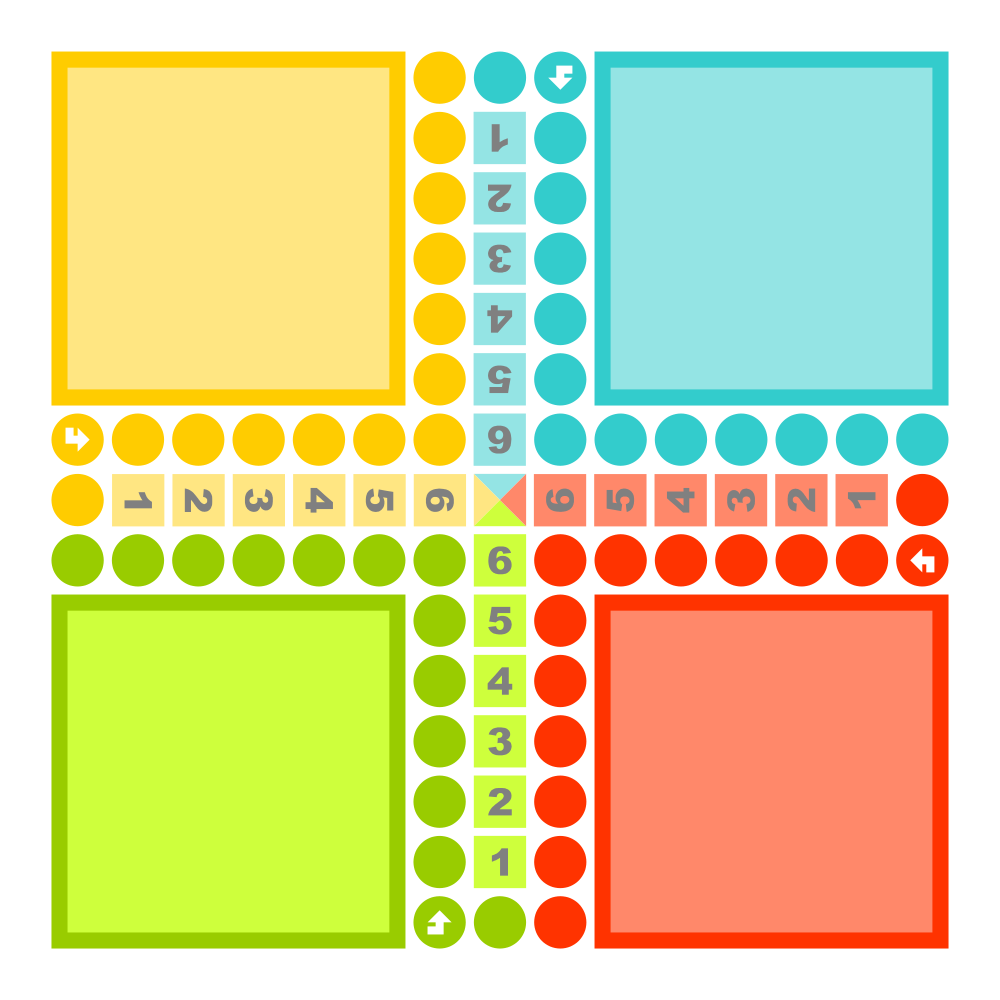
\includegraphics[scale=0.1888]{plateau.png}
        \caption{plateau}
    \end{minipage}
\end{figure}

\begin{figure}[h]
      \begin{minipage}[c]{.46\linewidth}
        \centering
        \includegraphics[scale=2]{lancer_le_dé.jpg} 
        \caption{bouton lancer dé}
    \end{minipage}
    \hfill%
     \hfill%
     \begin{minipage}[c]{.46\linewidth}
        \centering
        \includegraphics[scale=0.4]{Meilleurs-Scores-Grand.png}
        \caption{bouton meilleur scores}
    \end{minipage}
    \hfill%
     \begin{minipage}[c]{.46\linewidth}
        \centering
        
\includegraphics[scale=2]{nouvelle_partie.jpg}
        \caption{bouton nouvelle partie}
    \end{minipage}
     \hfill%
     \begin{minipage}[c]{.46\linewidth}
        \centering
        
\includegraphics[scale=2]{nouvelle_partie_enfonce.jpg}        \caption{bouton nouvelle partie}
    \end{minipage}
    \hfill%
    

    
\end{figure}

\newpage

\section*{ \Large\it{2- Premier squelette : } } 

\large{Avant de directement taper des lignes de code nous avons établi un squelette général de notre jeu , afin d'avoir une idée des fonctions primordiales à programmer. 
Le schéma général sur lequel on s'était entendu est représenté ci dessous : 
       \begin{figure}[h]
    \begin{minipage}[c]{.46\linewidth}
        \centering
        \includegraphics[scale=0.3]{Capture.png} 
       
    \end{minipage}
    \end{figure}
Biensûr , il y'aura beaucoup beaucoup de modifications pendant le codage , selon nos besoins , et aussi selon nos connaissances.}


\newpage
\section*{ \Large\it{3- Typedef :}} 

\large {Nous avons défini différents types qui seront essentiels a notre jeu : 
comme par exemple \newline
\color{red}Le type cheval}\color{black}  qui définit un pion avec sa position ( un entier x et un entier y ) , son avancement ( le nombre de cases qu'il a parcouru à l'instant T ) \newline
\color{red}{Le type joueur}\color{black}   qui possède 2 chevaux ( le cj1 et le cj2 de type cheval défini juste avant )  , une couleur , et une ecurie qui est initialisée à 2 vu que chaque joueurs possède 2 pions au départ ). 

\section*{ \Large\it{4- Fonctions principales :}}
\large{La fonction principale de notre jeu qui est d'ailleurs la première à laquelle on a commencer à reflechir est la fonction : 
\section*{ - avancer\_cheval :} 
Comme notre plateau de jeu est assez spécial , il a fallu étudier tous les cas possibles quelle que soit la position d'un pion sur les plateaux. 
Nous nous sommes donc intéressés aux coordonnées du pion , ça tombe bien car un pion ( un cheval ) est defini par un x et y qui indiquent sa position sur le plateau. 
Et ensuite selon sa position soit il bouge a gauche ( x--) , en haut (y--), en bas (y++) , ou a droite ( x++ ) .} 

\section*{ - est\_six :} 
\large{c'est une fonction qui étudie tous les cas possibles dans le cas où le joueur obtient un 6 après le lancer de dé. 
exemple: 
- lorsque  le joueur n'a encore aucun pion de sorti alors son pion 1 sort automatiquement 
- lorsque le joueur obtient un six et que son pion est vient tout juste de sortir ( il est donc sur sa case de départ ) et avance automatiquement de 6 cases car il ne peut pas faire sortir son 2ème pion. 
- lorsque le joueur a un pion sur le plateau ( hors case de départ ) et un pion dans son écurie , alors il a le choix entre faire avancer ce dernier , ou sortir l'autre 
- lorsque le joueur possède ses deux pions sur le plateau ( donc hors écurie ) on lui laisse également le soin de choisir lequel il veut faire avancer.}
\newpage

\section*{ - retour\_ecurie : }
\large{Elle remet tout simplement un cheval donné dans son écurie respective ( tout dépend donc de sa couleur ).
cette fonction est importante car elle est appellé lorsque deux pions ennemis se croisent ( on dit alors , qu'un pion en mange un autre  ).}

\section*{ - choix\_user2 : }
\large{Cette fonction est appellé dans la fonction est\_six. 
elle correspond au cas de figure où le joueur possède un pion hors case départ et un pion en écurie. 
Elle lui donne donc le choix de : soit avancer son cheval 
, soit en sortir un autre.
le choix se fait par un clic sur un des deux boutons qui apparaitront dans ce cas de figure et qui sont : 
sortir cheval / avancer cheval}

\section*{ - Choix\_user3 : }
\large{Est appellée quand les 2 pions du joueur  sont sur le plateau. 
il a donc la possibilité de cliquer sur le pion qu'il souhaite faire avancer. 
on récupère les coordonnées du clic et on les compare a celles des deux chevaux , pour déterminer lequel faire avancer.}

\section*{ - la fonction lancer\_dé :}
\large{elle retourne tout simplement un entier aléatoire entre 1 et 6 , son résultat est ensuite utilisé pour savoir de combien de cases nous allons avancer un cheval , ou si l'on doit en sortir un etc.. 
c'est pour cela que dans notre fonction principale nous ferons un : 
$l=lancer\_le\_de();$
et nous utiliserons l'entier l comme paramètre pour d'autres fonctions.}


\vspace*{3cm}
   
   
    \begin{minipage}{0.4\textwidth}
      \begin{flushright} \large
      
         \textsc{Merci de votre attention.}\\
      \end{flushright}
    \end{minipage}

\end{document}